\documentclass[journal]{IEEEtran}
\usepackage{graphicx}
\usepackage{caption}
\usepackage{subcaption}
\usepackage[nocompress]{cite}
\usepackage{amsmath, amsthm, amssymb}
\usepackage{enumerate}
\usepackage{url}
\usepackage{epstopdf}
\newtheorem{theorem}{Theorem}
\newtheorem{lemma}{Lemma}
\newtheorem{definition}{\bf Definition}
\newtheorem{remark}{Remark}

\theoremstyle{definition}
\newtheorem{example}{Example}

\usepackage{extarrows}
\usepackage{amsfonts}
\usepackage{algorithm, algorithmic}
\usepackage{color}
\usepackage{mathrsfs}
\usepackage{multirow}

\makeatletter
\newcommand{\ALOOP}[1]{\ALC@it\algorithmicloop\ #1
  \begin{ALC@loop}}
\newcommand{\ENDALOOP}{\end{ALC@loop}\ALC@it\algorithmicendloop}
\renewcommand{\algorithmicrequire}{\textbf{Input:}}
\renewcommand{\algorithmicensure}{\textbf{Output:}}
\newcommand{\algorithmicbreak}{\textbf{break}}
\newcommand{\BREAK}{\STATE \algorithmicbreak}
\makeatother


% *** GRAPHICS RELATED PACKAGES ***
%
\ifCLASSINFOpdf
\else
\fi

\hyphenation{op-tical net-works semi-conduc-tor}


\begin{document}    


\title{}%{Covert Communication in Joint Radar and Communication System}

%\author{
%\thanks{Zhixin Liu, Sainan Wang
%are with the Institute of Electrical Engineering, Yanshan
%University, Qinhuangdao 066004, China.
%}}

\markboth{Manuscript}{?}

\maketitle
%\begin{abstract}
%\end{abstract}
%\begin{keywords}
%\end{keywords}
\section{Introduction}
Important security information needs to be transmitted covertly to prevent it from being attacked
\begin{figure}[H]
\centering
\includegraphics[width=8.5cm]{model.eps}
\caption{System model.}
\label{F1}
\end{figure}
\section{Problem  Definition}
\subsection{System Model}
In this paper,We consider A IoV edge computing network, consisting of cloud computing layer, MEC layer,
as shown in Fig. 1. For MEC layer,which has moderate computation capacity and deploys close to networks, can be used to assist the vehicles. Cloud computing layer,can be used to process the large-scale, delay-insensitive data that MEC layer can not process��
��Reinforcement Learning����numerous vehicle-to-RSU (V2I) cells underlay a macrocell. in which each RSU
is equipped with a MEC server to provide computation offloading services to the vehicles��To avoid inter-cell interference, the time division multiple access (TDMA) communication technology is adopted. Time resource is divided into multi-frames, and each frame is divided into several time slots. Different VUEs access its time slots when they communicate with the RSU, and signal transmission in different time slots will produce no interference [10].��su03����We denote the set of users and MEC servers in the mobile system as U = {1, 2,...,U} and S = {1, 2,...,S}, respectively. ��joint��Some notations are given in Table I


\begin{table}[!h]\label{II}
\caption{Notations}
\centering
{\small\begin{tabular}{ll}
\hline
\hline
$\textrm{Pr}\{\cdot\}$ & Probability function. \\
$\mathbb{R}^n$         & Set of $n$-dimensional real vectors.\\
$\mathbb{E}\{\cdot\}$ &  Mathematical expectation of a random variable. \\
$\mathbb{D}\{\cdot\}$ &   Variance of a random variable. \\
$\mathcal{M}$  & Index set of all time slots $\mathcal{M}$$=$$\{1,2,\cdots,M\}$.\\
$\mathcal{I}$   & Index set of all active CMs $\mathcal{I}$$=$$\{1,2,\cdots,N\}$.\\
$\mathcal{J}$   & Index set of all CHs $\mathcal{J}$$=$$\{1,2,\cdots,N\}$. \\
\hline
\hline
\end{tabular}}
\end{table}

\subsection{Communication Model}
Different from the traditional cellular communication,Due to the fast mobility of vehicles, their CSIs are hard to be estimated precisely. In particular, RSU can only achieve the accurate knowledge of large-scale fading
of vehicular to RSU links while the small-scale fading $L_{v,m}^2$ of vehicular to RSU links while the small-scale fading $h_{v,m}\ $is greatly influenced by the fast channel variations caused by the Doppler effect. We assume that such CSIs is obtained through channel estimation , Therefore, we model the small-scale fading channel estimation of $h_{v,m}$by using the first-order Gauss�CMarkov process [27] in each TTI as follows
\begin{eqnarray}\label{E1}
h_{v,m}=\xi_{v,m}{\widetilde{h}}_{v,m}+\sqrt{1-\xi_{v,m}^2}\ \ \zeta_{v,m},
\end{eqnarray}
we assume that the estimated channel gain ${\widetilde{h}}_{v,m} $denotes the estimate of$ h_{v,m} $and  ${\widetilde{h}}_{k,m}^2 $is exponentially distributed with unit mean [33]. Furthermore, $\xi_{v,m}\epsilon\left(0,1\right)$represents the correlation coefficient over v �� m link, and $\zeta_{v,m}$stands for the channel gain and follows a complex Gaussian distribution $\zeta_{v,m}$~$CN\left(0,\delta^2\right)$.and independent and uncorrelated of ${\widetilde{h}}_{v,m}$. The coefficient $(0 <\zeta_{v,m}< 1) $quantifies the channel correlation between the two consecutive time slots and we assume that time correlation coefficient $\zeta_{v,m}$ is same for all VUEs. According to the Jakes statistical model for the fading channel [28], $\zeta_{v,m}$ is given as
$\zeta_{v,m}$=$J_{0}\left(2 \pi f_{\max } T_{s}\right)$(4)
where$ J_0$ is the zero-order Bessel function of the first kind. $f_{max} =\bar{\nu}f_c/c$ is the maximum Doppler frequency, where $\bar{\nu}$ indicates the vehicle speed, $f_c $indicates the carrier frequency, and$f_{max}$=$\bar{\nu}f_c/c$ ��
$T_s$ is a period feedback latency. Generally,both transmitter vehicles and RSU can know the accurate$ \zeta_{v,m}$.Based on the aforementioned discussion, the mobile V2I channel power gain of the effective links and interference links in kth time slot can be expressed as a shared expression:
\begin{eqnarray}\label{E2}
G_{v,m}^k={\hat{g}}_{v,m}^k+{\widetilde{g}}_{v,m}^k,
\end{eqnarray}
Where$ {\hat{g}}_{v,m}^k=L_{v,m}^2{\widetilde{h}}_{v,m}^2\xi_{v,m}^2$ ��$ {\widetilde{g}}_{v,m}^k=L_{v,m}^2\left(1-\xi_{v,m}^2\right)\ \ \zeta_{v,m}^2$ ,and $ {L_{v,m}^k}^2$denotes the kth time slot large-scale fading effects including shadow-fading and path loss fromith transmitter to jth receiver on the road section��Moreover, $ {\hat{g}}_{v,m}^k $is an observed value. ${\widetilde{g}}_{v,m}^k$ denotes an exponential random variable with parameter $E\left(\frac{1}{{L_{v,m}^k}^2\sqrt{1-{\zeta_{v,m}^k}^2}}\right)$.

To improve the spectrum utilization and realize multi-vehicles joint communication, V2I communications reuse the same uplink channel. In this case, the Signal-to-Interference-plus-Noise Ratio (SINR) from vehicle$ i $to RSU can be formulated as, $ \gamma_i^v=\frac{p_ig_{i,0}}{{\sum_{j=1,j\neq i}^{M}{p_jg_{j,0}}+\sigma}^2} $where pj denotes the transmit power of the jth vehicles��where ��2 is the background noise��Therefore, the deterministic equivalent transmission rate of VUEs calculated by Shannon��s theorem is$ {R_i\left(P\right)=log}_2{\left(1+\frac{p_ig_{i,0}}{{\sum_{j=1,j\neq i}^{M}{p_jg_{j,0}}+\sigma}^2}\right)}$,Hence, the transmission time of vehicle u when sending its task input$ d_u $in the uplink can be calculated as, $ t_{i,up}=\frac{d_{i,up}}{R_i\left(P\right)} $�� where W is the bandwidth of the reused channel. Therefore, the sum time of all V2I links can be formulated as$ W\sum_{i=1}^{N}{log}_2{\left(1+\frac{p_ig_{i,0}}{{\sum_{j=1,j\neq i}^{M}{p_jg_{j,0}}+\sigma}^2}\right)} $,And$ d_{i,up} $is the amount of input data including system settings, program codes, and input parameters ��which is necessary to transfer the program execution.

Communication delay is another significant index that affects the performance of wireless networks. The packets to V2I receivers must be in the queue before they transmit at the speed of$ R_i$. It is assumed that the process of a packet arriving at the ith V2I receiver is a Poisson process with parameter$ k_i$, and the length of the data packet obeys the exponential distribution of parameter $\tau_i$. Under the M/M/1 model [34], the relationship between the expected delay and transmission rate of the ith V2I links can be expressed as $D_i=\frac{1}{{\tau_iR}_i-k_i}$.
\subsection{Computing Model}

where $P_a$ is the radar transmit power of vehicle A, $\mathbf{x}_a$ is the transmitted signal by the radar of vehicle A.

The received signal at vehicle A is given by
\begin{eqnarray}\label{E2}
\mathbf{y}_a[i]\!=\!\sqrt{P_a}\alpha h_{ab}^2\mathbf{x}_a[i]+\sqrt{P_b}h_{ba}\mathbf{x}_b[i]\\
+\sqrt{P_J}h_{ja}\mathbf{x}_j[i]+\mathbf{n}_a[i],\notag
\end{eqnarray}
where $\alpha$ denotes the energy efficiency of reflection, $\mathbf{x}_b[i]$ is the transmitted signal by the tag on vehicle A.

For the link from vehicle A to vehicle B, we have the two hypotheses as
\begin{eqnarray}\label{E3}
\begin{array}{ll}
\mathcal{H}_0:\mathbf{y}_b[i]=\sqrt{P_J}h_{jb}\mathbf{x}_j[i]+\mathbf{n}_b[i] \\
\mathcal{H}_1:\mathbf{y}_b[i] = \sqrt{P_a}h_{ab}\mathbf{x}_a[i]+\sqrt{P_J}h_{jb}\mathbf{x}_j[i]+\mathbf{n}_b[i],
\end{array}
\end{eqnarray}

The signal-to-interference-plus-noise-ratio received at vehicle B is
\begin{eqnarray}\label{E4}
SINR_b=\frac{P_a|h_{ab}|^2}{P_J|h_{jb}|^2+\sigma_b^2}
\end{eqnarray}


The signal-to-interference-plus-noise-ratio received at vehicle A is
\begin{eqnarray}\label{E5}
SINR_a=\frac{(P_b+P_a\alpha|h_{ab}|^2)|h_{ba}|^2}{P_J|h_{ja}|^2+\sigma_a^2}
\end{eqnarray}
where $h_{ba}=h_{ab}$.
%Considering the actual communication channel gains are uncertain and different to obtain, the target outage threshold is introduced to guarantee the normal communication of FUs and the energy harvesting of ERs.
%Therefore, the optimization problem in the non-colluding scenario aiming to maximize the secrecy rate is formulated as\footnote{In the two scenarios the QoS constraint of MU will be added after the transformation of objective function to avoid the situation that the SINR of MU can not meet the requirement of communication when the number of FBS is large. In this case, the transmit of MU can be constrained and the complexity of the problem can be simplified.}

%\subsection {Problem Formulation}
The optimization problems (P1) and (P2)  aim to maximize the utility functions that are the difference of payoff (maximization of SINR) and the cost functions
(minimization of power). $\mu_1$, $\mu_2$, and $\mu_3$ are the cost prices of the offered powers ($P_a$, $P_b$, and $P_J$), respectively. For the problem (P1), it consider the link from vehicle A to B. The probability constraint in (P1) is an outage probability constraint, which ensure a reliable radar links. The constraint $\xi_{ab} \geq 1-\varepsilon_{ab}$ aims to transmit radar signal covertly, $\xi_{ab}$ is the error detection probability.
For problem (P2), it consider the echo link from the tag on vehicle B to A . The probability constraint in (P2) is an outage probability constraint, which ensure a reliable communication links. The constraint $\xi_{ba}\geq 1-\varepsilon_{ba}$ aims to transmit the mixed signal (radar plus communication signal) covertly, $\xi_{ba}$ is the error detection probability. $\varepsilon_a$, $\varepsilon_b$, $\varepsilon_{ab}$, and $\varepsilon_{ba}$ are the very small probability thresholds.
\begin{equation}
{R_i\left(P\right)=log}_2{\left(1+\frac{p_ig_{i,0}}{{\sum_{j=1,j\neq i}^{M}{p_jg_{j,0}}+\sigma}^2}\right)}
\end{equation}
\begin{eqnarray}\label{E6}
\begin{array}{rll}
\textbf{P1}:&\max \ {R_i\left(P\right)=log}_2{\left(1+\frac{p_ig_{i,0}}{{\sum_{j=1,j\neq i}^{M}{p_jg_{j,0}}+\sigma}^2}\right)}\\
s.t.&\left\{
\begin{array}{lll}
&0\leq P_a\leq P_{a,max},\\
&\textrm{Pr} \{SINR_b\geq SINR_{b,min}\}\geq 1-\varepsilon_b,\\
&\xi_{ab} \geq 1-\varepsilon_{ab}
\end{array}
\right.
\end{array}
\end{eqnarray}

\begin{eqnarray}\label{E6}
\begin{array}{rll}
&\max \limits_{P_J} \,\,U_J=-SINR_b-\mu_3P_J   \\
&s.t. \ 0\leq P_J\leq P_{J,max},
\end{array}
\end{eqnarray}
\begin{eqnarray}\label{E7}
\begin{array}{rll}
\textbf{P2}:&\max \limits_{P_b} \,\,U_C=\ln(SINR_a-SINR_{a,min})-\mu_2(P_a+P_b\alpha|h_{ab}|^2)\\
s.t.&\left\{
\begin{array}{lll}
&0\leq P_b\leq P_{b,max},\\
&\textrm{Pr} \{SINR_a\geq SINR_{a,min}\}\geq 1-\varepsilon_a,\\
&\xi_{ba}\geq 1-\varepsilon_{ba}
\end{array}
\right.
\end{array}
\end{eqnarray}
The shortcomings of these problems are that the channel uncertainty is not considered in the objective functions. I will consider it with the help of the characteristic of radar signal.
Moreover, the transformations of the covert communication constraints need to have a detailed derivation.
Through problem (P1), we can obtain an equality relation between $P_R$ and $P_J$ if the convex optimization theory can be applied to.
%\ifCLASSOPTIONcaptionsoff
%  \newpage
%\fi
%\begin{thebibliography}{1}
%\end{thebibliography}
\subsection {Preliminaries}
As a novel parametrization of radar
performance, radar estimation rate (radar mutual information) has been mentioned in many works \cite{ARChiriyath}-\cite{AAhmed}.  The estimation rate is a metric analogous to the communications rate and provides
a measure of the information about a target (range, cross-section, shape, roughness or moisture level) that is gained from radar illumination in radar tracking estimation scenarios.
 In general, the target has some entropy or information
about itself that is not explicitly being communicated to the
radar system by the target. Radar illumination can be viewed
as the target unwillingly communicating this target entropy
or information to the radar receiver. Thus, this information rate is constructed by
considering the entropy of a random parameter being estimated
and the entropy of the estimation uncertainty of that parameter, and the radar channel can be characterized as an uncooperative communications channel \cite{ARChiriyath}.

Generally, waveform optimization is necessary for detection and target information extraction. Especially, the radar waveform is designed so as to maximize the mutual information (MI) between the target parameter of interest and the measurements obtained from the receiver \cite{ARChiriyath2}.

To improve the spectrum utilization efficiency and achieve the low cost of hardware, signal-sharing is the most popular approach used in joint radar and
communication (JRC) systems. There are two commonly used dual function signals, i.e,  Frequency-Modulated Continuous Wave (FMCW) signal and Orthogonal Frequency Division Multiplexing (OFDM) signal \cite{NCLuong}.
It is noted that FMCW is a type of linear
frequency modulation (LFM) or chirp modulation in which the frequency increases or decreases with a so-called chirp rate \cite{CHW}. As for the radar function, it has
also been been pointed out in another study \cite{GFranken} that OFDM coded radar signals are comparable with LFM signals and furthermore, experiences no range-Doppler coupling \cite{YLSit}. Besides, the OFDM has several other advantages such as robustness against multipath fading, easy synchronization and equalization, and high flexibility \cite{NCLuong}. These advantages enable the OFDM to be effectively used for the target detection of the radar function.

 Given that these advantages of OFDM signal and the radar estimation rate which is  analogous to the communications data rate, many OFDM-based JRC systems \cite{KWHuang}-\cite{AAhmed} are considered to perform waveform design by maximizing the MI between target impulse response and the received signal.

In \cite{ARChiriyath2}, the involved JRC system does not explicitly state the type of signal. The JRC system consists of an active, mono-static, pulsed radar and a single-user communications system. The authors consider the
 JRC receiver to be a radar transmitter/receiver that can act as a communications receiver. The joint receiver can simultaneously estimate the radar target parameters from the radar return and decode a received communications signal.
In this scenario, the JRC system acts as a dual functional receiver, and the sources of the radar return signal and the communication signal are separated (from target and communication user, respectively). However, \cite{ARChiriyath2} only derives achievable bounds on performance for a receiver that observes communications and radar return in the same frequency allocation, the corresponding optimization problem is omitted. To integrate covert communications into this JRC system, we can introduce a jammer here to prevent the effective detection from the warden.

Besides, OFDM signal-based related works \cite{KWHuang}-\cite{MBicaK} proposed different Mutual Information based criteria for radar waveform optimization and  formulated the corresponding waveform optimization problems. However, these works consider the coexistence of radar and communication systems in the same spectrum, instead of dual-functional radar-communications (DFRC) system. Moreover, the OFDM signal is early processed to facilitate the MI-based waveform design problem. There is a need to learn the corresponding knowledge of signal processing. After that, the optimization problem which maximizes the MI with interference constraints can be easily obtained.

In \cite{AAhmed}, a dual-purpose
OFDM transmitter is exploited which optimizes the transmit
power of different sub-carriers to fulfill the radar objectives.
These OFDM sub-carriers used by the radar are also allocated to different communication receivers to achieve the communications objectives (like D2D communication networks). The MI between the frequency-dependent target response and the transmit waveform is used as the optimization objective for radar performance.
The communication performance is optimized by allocating the
radar sub-carriers to different communication users by using MI
maximization as the criterion. The resulting optimization problem maximizing the MI for radar can be simplified a standard convex optimization. This work provides the most popular system framework.
\subsection {Vehicle Computation Task}
 We consider that each vehicle $u\in U$ has one computation task at a time. denoted as Tu , that is atomic and cannot be divided into subtasks. Each computation task Tu is characterized by a tuple of two parameters.I plan to have the detailed formula derivation for these works \cite{KWHuang}-\cite{AAhmed}, and formulate a reasonable system model .






The channels of RFE-PR, RFE-Tag, RFE-AR, Jammer-PR, Jammer-Tag, Jammer-AR, Tag-PR and Tag-AR are denoted by $g_{sw}$, $g_{st}$, $g_{sr}$, $g_{jw}$, $g_{jt}$, $g_{jr}$, $h_{tw}$ and $h_{tr}$, respectively.  Since the links of Tag-PR and Tag-AR operate over short distances,  $h_{tw}$ and $h_{tr}$ are assumed to meet the following channel model:
\begin{eqnarray}\label{}
h_{ij}=\hat{h}_{ij}+\tilde{h}_{ij}
\end{eqnarray}
where $ij$$\in$$\{tw, tr\}$. $\hat{h}_{ij}$ and $\tilde{h}_{ij}$ denote the estimated part and the deviation. They are zero-mean, independent, CSCG random variables. Their variances satisfy $\mathbb{E}[|\hat{h}_{ij}|^2] =K_{ij}\beta$ and
$\mathbb{E}[|\tilde{h}_{ij}|^2]=K_{ij}(1-\beta)$ to ensure the total power of $h_{ij}$ is $K_{ij}$.


The remaining long-distance links are assumed to follow Rayleigh fading and the corresponding average channel gains denote $\varphi_{kl}$, where $kl$$\in$$ \{sw,st,sr,jw,jt,jr\}$. (Could I assume that all $\varphi_{kl}$ is approximately equal since these long distances can be regarded as nearly equal in length?)


In this model, the backscatter signal reflected by tag is given by
\begin{eqnarray}\label{E9}
\mathbf{x}(i)= \left(\sqrt{\alpha P}g_{st}\mathbf{e}(i)+\sqrt{\alpha J}g_{jt}\mathbf{j}(i)\right)\mathbf{s}(i),
\end{eqnarray}
where $i$$=$$1,2,\ldots, n$ is the index of each channel use, $\alpha$ is Tag's reflection coefficients for the signals from RF emitter and jammer. $P$ and $J$ are the transmit powers of RF emitter and jammer, respectively. The $i$-th elements of vector $\mathbf{e}$ and $\mathbf{j}$, $\mathbf{e}(i)$ and $\mathbf{j}(i)$, denote the signals emitted at RF emitter and jammer for the $i$-th channel use, respectively,  while $\mathbf{s}(i)$ is the signal modulated at Tag. Note that $\mathbb{E}[\mathbf{e}(i)\mathbf{e}^{*}(i)]$$=$$1$, $\mathbb{E}[\mathbf{j}(i)\mathbf{j}^{*}(i)]$$=$$1$ and $\mathbb{E}[\mathbf{s}(i)\mathbf{s}^{*}(i)]$$=$$1$.(Could I here assume that the jammer signal is completely absorbed by Tag so that there are less energy to be detected and then ensure a good covert communication? However, the fact is that the reflection coefficients always be the same when there are several signals to be scattered at the same time.)

 The received signal at AmBC receiver is given by
\begin{eqnarray}\label{E10}
\mathbf{y}_r(i)\!=\! h_{tr}\mathbf{x}(i)\!+\!\left(\sqrt{\phi P}g_{sr}\mathbf{e}(i)\!+\!\sqrt{\phi J}g_{jr}\mathbf{j}(i)\right)\!+\!\mathbf{n}_r (i),
\end{eqnarray}
where $\mathbf{n}_r (i)$ is the additive white Gaussian noise (AWGN) at
AmBC receiver with zero mean and the variance of $\sigma_r^2$,  $\phi\in[0,1]$ is the interference cancellation coefficient and $\phi$$=$$0$ means
the perfect interference cancellation.

 The composite received signal at PR of
observation vector $\mathbf{y}_r$ for the $i$-th channel use is given by

\begin{equation}\label{E11}
\mathbf{y}_w(i)\!=\!
\left\{
\begin{array}{ll}
\!\sqrt{P}g_{sw}\mathbf{e}(i)\!+\!\sqrt{J}g_{jw}\mathbf{j}(i)\!+\!\mathbf{n}_w (i), &\!\mathcal{H}_0, \\
\!\sqrt{P}g_{sw}\mathbf{e}(i)\!+\!\sqrt{J}g_{jw}\mathbf{j}(i)\!+\!\mathbf{x}(i)h_{tw}\!+\!\mathbf{n}_w (i) ,&\!\mathcal{H}_1,
\end{array}
\right.
\end{equation}
or
\begin{equation}\label{E12}
\mathbf{y}_w(i)\!=\!\!
\left\{
\begin{array}{*{20}ll}
\!\!\!\sqrt{P}g_{sw}\mathbf{e}(i)\!\!+\!\!\sqrt{J}g_{jw}\mathbf{j}(i)\!\!+\!\!\sqrt{\alpha J}g_{jt}\mathbf{j}(i)h_{tw}\!\!+\!\!\mathbf{n}_w (i), &\!\!\!\mathcal{H}_0, \\
\!\!\!\sqrt{P}g_{sw}\mathbf{e}(i)\!\!+\!\!\sqrt{J}g_{jw}\mathbf{j}(i)\!\!+\!\!\mathbf{x}(i)h_{tw}\!\!+\!\!\mathbf{n}_w (i) ,&\!\!\!\mathcal{H}_1,
\end{array}
\right.
\end{equation}
We consider equal prior probability of $\mathcal{H}_0$ and $\mathcal{H}_1$ here. Let  $P_{FA}$ and $P_{MD}$ denote the probabilities of
false alarm and missed detection, respectively. Hence, PR's total probability of detection error $\xi$ can be given by,
\begin{eqnarray}\label{E11}
\xi=P_{FA}+P_{MD},
\end{eqnarray}
where $P_{FA}$$=$$\mathbf{Pr}\{D_1|\mathcal{H}_0\}$ and $P_{MD}$$=$$ \mathbf{Pr}\{D_0|\mathcal{H}_1\}$. Due to the binary hypothesis detection, $D_1$ and $D_0$ represent the binary decisions that infer whether Tag reflects or not, respectively.
\begin{eqnarray}\label{}
P_w \mathop{\gtrless}\limits_{D_0}^{D_1}\tau,
\end{eqnarray}
where $\tau$ is the energy detection threshold of PR.

$P_w=\frac{1}{n}\sum\nolimits_{i=1}^{n}|\mathbf{y}_w(i)|^2$.

Specifically, there are two cases.

a)
\begin{equation}\label{E12}
P_w\!=\!
\left\{
\begin{array}{ll}
\!\!\!P|g_{sw}|^2\!+\!\!J|g_{jw}|^2\!+\!\sigma_w^2, &\!\!\!\mathcal{H}_0, \\
\!\!\!P|g_{sw}|^2\!+\!\!J|g_{jw}|^2\!+\!\alpha(P|g_{st}|^2\!+\! J|g_{jt}|^2)|h_{tw}|^2\!+\!\sigma_w^2,&\!\!\!\mathcal{H}_1,
\end{array}
\right.
\end{equation}
or

b)
\begin{equation}\label{}
P_w\!=\!
\left\{
\begin{array}{ll}
\!\!\!P|g_{sw}|^2\!+\!\!J|g_{jw}|^2\!+\!\alpha J|g_{jt}|^2|h_{tw}|^2\!+\!\sigma_w^2, &\!\!\!\mathcal{H}_0, \\
\!\!\!P|g_{sw}|^2\!+\!\!J|g_{jw}|^2\!+\!\alpha( P|g_{st}|^2\!+\! J|g_{jt}|^2)|h_{tw}|^2\!+\!\sigma_w^2,&\!\!\!\mathcal{H}_1,
\end{array}
\right.
\end{equation}
where case a) illustrates the binary decisions that inferring  whether Tag reflects the mixed signals or not, while case b) shows the binary decisions that inferring  whether Tag transmits information based on the single RF signal.

Minimizing sum of error probabilities

For case a), the equivalent noise power forms at PR under $\mathcal{H}_0$ is
\begin{eqnarray}\label{}
\sigma_w^{\prime2}=\tilde{\sigma}_w^2+\sigma_w^2
\end{eqnarray}
where $\tilde{\sigma}_w^2$$=$$P|g_{sw}|^2+J|g_{jw}|^2$, which follows generalized chi-squared distribution with the corresponding probability density function (PDF) derived from \cite{DHamma}.
\begin{eqnarray}\label{E18}
f(x;m,\lambda_1,\lambda_2,\ldots,\lambda_m)=\sum\limits_{i=1}^m a_i\exp\left(-\frac{x}{\lambda_i}\right),
\end{eqnarray}
where
\begin{eqnarray}\label{E19}
a_i=\frac{1}{\lambda_i\prod\nolimits_{j=1,j\neq i}^m(1-\lambda_j/\lambda_i)}.
\end{eqnarray}
Under $\mathcal{H}_0$ in case a), we have $m=2$, and
\begin{eqnarray}\label{}
\left(\lambda_1,\lambda_2\right)=(\mu,\nu).
\end{eqnarray}
where $\mu$$=$$P\varphi_{sw}$, $\nu$$=$$J\varphi_{jw}$.
It is noted that the transmit power of RF emitter $P$ is always higher than the transmit power jammer $J$ in the real scenes.
Hence, when $\tau>\sigma_w^2$, $P_{FA}(\tau)$ can be determined through
\begin{eqnarray}\label{}
\begin{array}{lll}
P_{FA}(\tau)&= \mathbf{Pr}\{\sigma_w^{\prime2}>\tau-\sigma_w^2\}\\
&=\sum\limits_{i=1}^2a_i\lambda_i\exp\left(-\frac{\tau-\sigma_w^2}{\lambda_i}\right)\\
&=\frac{\mu\exp(-\frac{\tau-\sigma_w^2}{\mu})-\nu\exp(-\frac{\tau-\sigma_w^2}{\nu})}{\mu-\nu} .
\end{array}
\end{eqnarray}
Eventually, the false alarm probability can be formulated as
\begin{eqnarray}\label{}
P_{FA}(\tau)=
\left\{
\begin{array}{ll}
1, \tau\leq\sigma_w^2\\
\frac{\mu\exp(-\frac{\tau-\sigma_w^2}{\mu})-\nu\exp(-\frac{\tau-\sigma_w^2}{\nu})}{\mu-\nu} ,\tau>\sigma_w^2
\end{array}
\right.
\end{eqnarray}
\begin{figure}[hptb!]
\centering\small
\includegraphics[width=8cm]{figurec.eps}
\caption{ Secondary user data transmission rate under different numbers.}
\end{figure}

Similarly, the missed detection probability is formulated as

\begin{eqnarray}\label{}
P_{MD}(\tau)=\mathbf{Pr}\{\tilde{\sigma}_w^2\!+\!\alpha( P|g_{st}|^2\!+\! J|g_{jt}|^2)|h_{tw}|^2\!+\!\sigma_w^2\leq\tau\}.
\end{eqnarray}
Let $\theta$$\triangleq$$\tilde{\sigma}_w^2\!+\!\alpha( P|g_{st}|^2\!+\! J|g_{jt}|^2)K\!$, $K$$=$$|h_{tw}|^2$.
Under $\mathcal{H}_1$ in case a), we have $m=4$, and
\begin{eqnarray}\label{}
\left(\lambda_1,\lambda_2,\lambda_3,\lambda_4\right)=(\mu,\nu,\alpha K\omega,\alpha K\pi).
\end{eqnarray}
where $\omega$$=$$P\varphi_{st}$, $\pi$$=$$J\varphi_{jt}$.
Based on  \eqref{E18} and \eqref{E19}, $P_{MD}(\tau)$ is reformulated as
\begin{eqnarray}\label{}
P_{MD}(\tau)=
\left\{
\begin{array}{ll}
0, \tau\leq\sigma_w^2\\
\sum\limits_{i=1}^4\left[a_i\lambda_i-a_i\lambda_i\exp\left(-\frac{\tau-\sigma_w^2}{\lambda_i}\right)\right],\tau>\sigma_w^2
\end{array}
\right.
\end{eqnarray}
where $a_1$$=$$\frac{P/\varphi_{sw}}{(P-J)(1-\alpha K)(P-\alpha KJ)}$, $a_2$$=$$\frac{J/\varphi_{jw}}{(J-P)(J-\alpha KP)(1-\alpha K)}$,\\
$a_3$$=$$\frac{P/\varphi_{st}}{(1-\frac{1}{\alpha K})(\alpha KP-J)(P-J)}$, and
$a_4$$=$$\frac{J/\varphi_{jt}}{(\alpha KJ-P)(1-\frac{1}{\alpha K})(J-P)}$, if $\varphi_{sw}$$\approx$$\varphi_{jw}$$\approx$$\varphi_{st}$$\approx$$\varphi_{jt}$. (Based on these, the monotonicity of $P_{MD}(\tau)$ is hard to determined when $m$$=$$4$. Most of the existing papers only consider the case of $m$$=$$2$. )

Through my calculation, I find that $\sum\nolimits_{i=1}^4a_i\lambda_i=1$, $a_1>0$, $a_2>0$, $a_3<0$, and $a_4<0$ when $\alpha KP>J$(i.e., the effective backscatter transmission from RF emitter to AmBC receiver is stronger than the direct link from jammer).


To capture the optimal detection threshold at the minimum total error probabilities, we need to solve the problem as follows
\begin{eqnarray}\label{}
\min\limits_\tau\xi
\end{eqnarray}
\subsection {Next task}
 If there are no better solution, I will try the another method based on the existing system model. Here, the channel uncertainty can be dismissed and the uncertain power obeying the distribution in (18) and (19) can be considered, since there are exactly two power variables (i.e., the power of RF emitter and the power of jammer) .

\begin{thebibliography}{60}
\bibitem{DHamma}
 D. Hammarwall, M. Bengtsson, and B. Ottersten, ``Acquiring partial
CSI for spatially selective transmission by instantaneous channel norm
feedback'', \emph{IEEE Trans. Signal Process}., vol. 56, no. 3, pp. 1188�C1204,
Mar. 2008.
\end{thebibliography}
\end{document}

